%% -*- coding:utf-8 -*-
\begin{figure}
\centering
\ifpdf
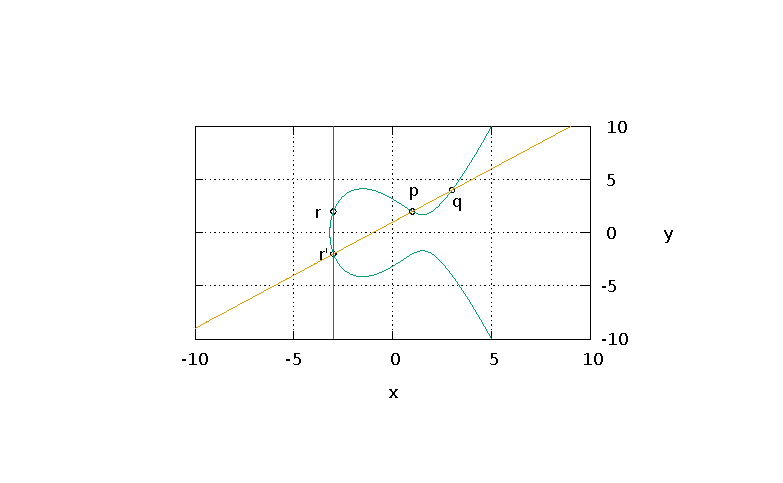
\includegraphics[angle=0,scale=1.5]
{./add/discretmath/picellipticsum.pdf}
\else
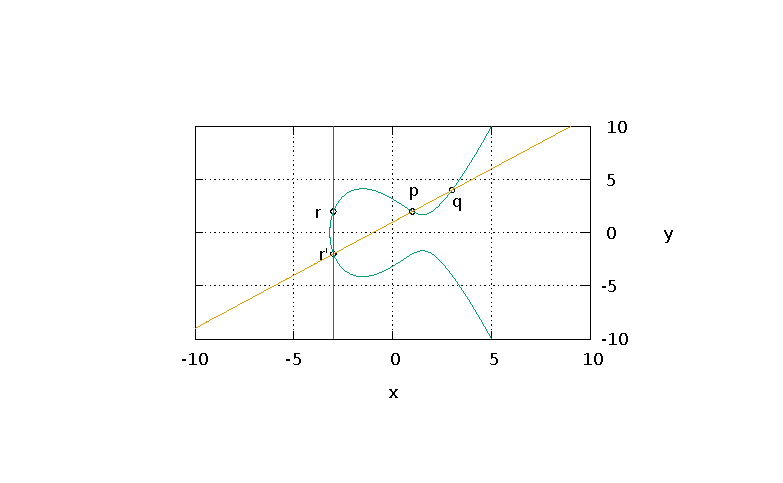
\includegraphics[angle=0,scale=1.5]
{./add/discretmath/picellipticsum.eps}
\fi
\caption{Эллиптическая кривая $y^2 = x^3 -7 x + 10$ над полем
  вещественных чисел $\mathbb{R}$. Сложение двух точек $p(1,2)$ и
  $q(3,4)$. Прямая проходящая через эти точки пересекает кривую еще в
  третьей точке $r'(-3,-2)$. Симметричная $r'$ относительно кривой
  точка $r(-3,2)$ является суммой исходных двух: $p + q = r$}
\label{fig:add:ellipticRsum}
\end{figure}
